\section{Alternating Bit Protocol - modelling, specification and testing}
% no \IEEEPARstart
The alternating bit protocol is a simple yet effective protocol (usually used as a test case), designed to ensure reliable communication through unreliable transmission mediums, and it�s used for managing the retransmission of lost messages \cite{ReactiveSystems3}\cite{Kulick}.

The representation of Alternating Bit Protocol is shown bellow, and it consists of $Sender$ $S$, $Receiver$ $R$ and two channels $Transport$ $T$ and $Acknowledge$ $A$. In the following text Alternating Bit Protocol is abbreviated as ABP.

\begin{figure}[!ht]
\centering
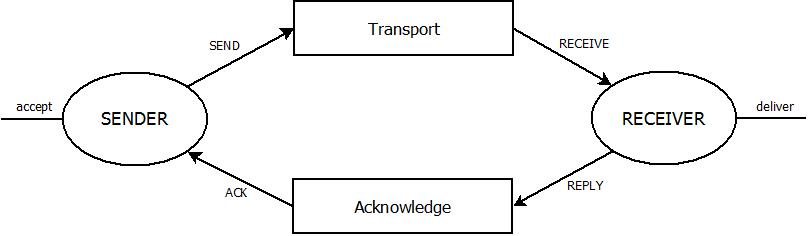
\includegraphics[width=4.5in]{abp}
\caption{Alternating bit protocol}
\label{fig:abp}
\end{figure}

All of the transitions in the ABP are internal synchronization and the only visible transitions are deliver and accept, which can occur only sequentially. 

Here is the specification of ABP:\\
$ABP=\overline{deliver}.accept.ABP$

Messages are sent from a sender $S$ to a receiver $R$. Channel from $S$ to $R$ is initialized and there are no messages in transit. There is no direct communication between the sender $S$ and the receiver $R$, and all messages must travel trough the medium (transport and acknowledge channel). The ABP works like this:
\begin{enumerate}
	\item Each message sent by $S$ contains the protocol bit, 0 or 1.\\
	      Here is the implementation:\\
	      $\left(S|T|R|A\right)\backslash \left(send0,send1,receive0,receive1,reply0,reply1,ack0,ack1\right)$
	\item When a sender $S$ sends a message, it sends it repeatedly (with its corresponding bit) until receiving an acknowledgment ($ack0$ or $ack1$) from a receiver $R$ that contains the same protocol bit as the message being sent.\\
	      $S=\overline{send0}.S+ack0.accept.S_{1}+ack1.S$\\
	      $S_{1}=\overline{send1}.S_{1}+ack1.accept.S+ack0.S_{1}$\\
	      The transport channel transmits the message to the receiver, but it may lose the message (lossy channel) or transmit it several times (chatty channel).
	      $T=send0.\left(T+T_{1}\right)+send1.\left(T+T_{2}\right)$\\
	      $T_{1}=\overline{receive0}.\left(T+T_{1}\right)$\\
	      $T_{2}=\overline{receive1}.\left(T+T_{2}\right)$
  \item When $R$ receives a message, it sends a reply to $S$ that includes the protocol bit of the message received. When a message is received for the first time, the receiver delivers it for processing, while subsequent messages with the same bit are simply acknowledged.
        $R=receive0.\overline{deliver}.R_{1}+\overline{reply1}.R+receive1.R$\\
        $R_{1}=receive1.\overline{deliver}.R+\overline{reply0}.R_{1}+receive0.R_{1}$\\
        Again the acknowledgement channel sends the ack to sender, and it also can acknowledge it several times or lose it on the way to the sender.\\
        $A=reply0.\left(A+A_{1}\right)+reply1.\left(A+A_{2}\right)$\\
        $A_{1}=\overline{ack0}.\left(A+A_{1}\right)$\\
        $A_{2}=\overline{ack1}.\left(A+A_{2}\right)$
  \item When $S$ receives an acknowledgment containing the same bit as the message it is currently transmitting, it stops transmitting that message, flips the protocol bit, and repeats the protocol for the next message.\cite{Kulick}\cite{ProcessAlgebraParallel}
\end{enumerate}

L = \left{send0,send1,receive0,receive1,reply0,reply1,ack0,ack1\right}

\begin{table}
\begin{tabular}{| p{15.5cm} | p{15.5cm} | }

	
  \hline                       
	ABP implementation state &
	ABP specification state	
	\\ \hline
	
\left[\left(\left(\left(\left(S\right)|\left(T\right)\right)|\left(R\right)\right)|\left(A\right)\right)\backslash,
\left(\left(\left(\left(S\right)|\left(\left(T\right)+\left(T1\right)\right)\right)|\left(R\right)\right)|\left(A\right)\right)\backslash,
\left(\left(\left(\left(S\right)|\left(\left(T\right)+\left(T1\right)\right)\right)|\left(R\right)\right)|\left(\left(A\right)+\left(A2\right)\right)\right)\backslash,
\left(\left(\left(\left(S\right)|\left(T\right)\right)|\left(R\right)\right)|\left(\left(A\right)+\left(A2\right)\right)\right)\backslash,
\left(\left(\left(\left(S\right)|\left(\left(T\right)+\left(T1\right)\right)\right)|\left(_deliver.\left(R1\right)\right)\right)|\left(A\right)\right)\backslash,
\left(\left(\left(\left(S\right)|\left(\left(T\right)+\left(T1\right)\right)\right)|\left(_deliver.\left(R1\right)\right)\right)|\left(\left(A\right)+\left(A2\right)\right)\right)\backslash,
\left(\left(\left(\left(S1\right)|\left(\left(T\right)+\left(T1\right)\right)\right)|\left(R1\right)\right)|\left(\left(A\right)+\left(A1\right)\right)\right)\backslash,
\left(\left(\left(\left(S1\right)|\left(\left(T\right)+\left(T2\right)\right)\right)|\left(_deliver.\left(R\right)\right)\right)|\left(\left(A\right)+\left(A1\right)\right)\right)\backslash,
\left(\left(\left(\left(S1\right)|\left(\left(T\right)+\left(T2\right)\right)\right)|\left(R1\right)\right)|\left(\left(A\right)+\left(A1\right)\right)\right)\backslash,
\left(\left(\left(\left(S\right)|\left(\left(T\right)+\left(T2\right)\right)\right)|\left(R\right)\right)|\left(\left(A\right)+\left(A2\right)\right)\right)\backslash\right] &
  ABP   
  \\ \hline
  
  \left[\left(\left(\left(\left(accept.\left(S1\right)\right)|\left(\left(T\right)+\left(T1\right)\right)\right)|\left(R1\right)\right)|\left(\left(A\right)+\left(A1\right)\right)\right)\backslash,
\left(\left(\left(\left(S\right)|\left(\left(T\right)+\left(T1\right)\right)\right)|\left(R1\right)\right)|\left(\left(A\right)+\left(A1\right)\right)\right)\backslash,
\left(\left(\left(\left(S\right)|\left(\left(T\right)+\left(T1\right)\right)\right)|\left(R1\right)\right)|\left(\left(A\right)+\left(A2\right)\right)\right)\backslash,
\left(\left(\left(\left(S\right)|\left(\left(T\right)+\left(T1\right)\right)\right)|\left(R1\right)\right)|\left(A\right)\right)\backslash,
\left(\left(\left(\left(S1\right)|\left(\left(T\right)+\left(T2\right)\right)\right)|\left(R\right)\right)|\left(\left(A\right)+\left(A2\right)\right)\right)\backslash,
\left(\left(\left(\left(accept.\left(S\right)\right)|\left(\left(T\right)+\left(T2\right)\right)\right)|\left(R\right)\right)|\left(\left(A\right)+\left(A2\right)\right)\right)\backslash,
\left(\left(\left(\left(S1\right)|\left(\left(T\right)+\left(T2\right)\right)\right)|\left(R\right)\right)|\left(\left(A\right)+\left(A1\right)\right)\right)\backslash\right] &
  ABP'
  \\ \hline  
  
\end{tabular}
\caption{Results of the comperisons}
\label{table3}
\end{table}


